%% APPENDIX B -- the spatial rank as a diagnostic: what it can and cannot
%% support, and the reserved hold-out that calibrates it.
%% Owner: r11-chain.  Carries \label{app:radius} (cited by 04_method.tex)
%% and \label{sec:heldout} (cited from the other appendices).
\section{The spatial rank, and what it can support}
\label{app:radius}

The spatial rank asks whether an excess sits at the star or anywhere else in
the field. It is a diagnostic, no disposition rests on it, and this appendix
is the measurement that settles why: \rankstatus{}

The star lies at the phase centre, inside the control annulus, and the
asymmetry is real. \emph{It is not a primary-beam effect.} Spectra are
extracted from phase-rotated visibilities in apparent flux and are never
corrected for the primary-beam response (Appendix~\ref{app:conventions}), so
the familiar rise of image noise with distance from the pointing centre
cannot operate here; were it operating it would make the control probes
noisier than the star and place the stellar rank \emph{above} one half, the
opposite of what is measured. What the control ensemble does show is a weak
rise of its own level with radius, and the obvious repair is to remove it:
each probe is standardised within its own radius bin, with no free parameter.

\emph{Applied out of sample, the correction does not repair the statistic.}
Frozen --- probe radii, bin edges and standardisation alike --- and applied
unmodified to \RadValStarN{} windows that played no part in its construction,
it moves the median stellar rank from \RadValStarRawMed{} to
\RadValStarCorMed{} against the exchangeable one half, \RadValStarToward{}
it, in both out-of-sample partitions separately; rescoring the whole survey
with the gradient removed moves the crossings outranking all their controls
from \LocStageGlobal{} windows to \LocStageLocal, and leaves the survey
median rank slightly further from one half than before. The gradient is real
but the residual is not radial, and neither normalisation yields a calibrated
tail probability, so we keep the frozen rank and rest every disposition on
physical evidence or on recurrence.

\emph{A calibration error that varied with frequency would explain the
displacement, and it is the only mechanism on offer.} An error identical in
every channel is removed exactly by the per-integration median along
frequency; a channel-dependent one is not, and two ordinary errors are
channel-dependent: a residual in the bandpass, and a system temperature
measured in the coarse correlator mode and interpolated onto the science
channels, which near a telluric line leaves a narrow feature behind
\citep{ALMATsys2018}. Both
multiply the continuum, so both act at the star and not on empty sky, both
stand still in topocentric frequency and both are coherent between
integrations: they would stack at near-zero drift and put the stellar rank
\emph{below} one half, the sign observed.

\emph{Amplitude alone does not exclude them.} What such an error multiplies
is the whole continuum at the extraction position, a dirty-map amplitude that
includes any dust inside the synthesised beam; what it must beat is the noise
of the de-drifted, block-combined spectrum, since a coherent residual stacks
as a carrier does. A fractional error $\epsilon$ deposits $\epsilon S_{\rm c}$
at the star, so a crossing at the trigger needs $\epsilon=5\sigma/S_{\rm c}$.
The survey's own continuum maps --- \CxNMap{} of them, each used only on
windows of its own band --- give \CxContMax\,mJy at \CxContMaxStar, a
\CxContMaxSnr$\sigma$ detection and a factor $\CxRatioHi$ above that star's
photosphere; on the measured continuum \CxNAdmit{} windows of
\CxNAdmitStar{} stars need only \CxEpsAdmitLoPct--\CxEpsAdmitHiPct{} per
cent, inside the \CdSpecTsysLo--\CdSpecTsysHi{} per cent a coarse system
temperature is known to leave at an ozone line; and at \CxAuStar, where the
same extractor measures \CxAuContMJy\,mJy near \CxAuGHz\,GHz,
\CxAuEpsPct{} per cent would suffice.

\emph{Those windows measure the residual instead, and it is too small.} In
all \CxNAdmit{} of them the largest statistic anywhere --- every channel,
every drift --- is $T_\star=\CxAdmitTstarHi$ where the trigger is five, the
largest control probe \CxAdmitCtrlHi, and \CxAdmitNCrossWord{} holds a
crossing. Read as
a fraction of the continuum beside it, the coherent channel-dependent
residual at the extraction position is below \CxResidHiPct{} per cent in all
of them and below \CxResidBestPct{} per cent at \CxResidBestStar, whose
continuum was measured in the one execution block its windows come from ---
beneath the \CdSpecTsysLo{} per cent floor of the documented range. Their
median stellar rank, \CxAdmitRankMed, lies on the far side of one half from
the displacement the mechanism is invoked to explain. \CxOneStar{} carries
the whole pattern within one star: \CxOneStarNAdmit{} of its windows would
admit \CxOneStarEpsLoPct--\CxOneStarEpsHiPct{} per cent and none produces
anything, while its one crossing lies in the window where
\CxOneStarCrossEpsPct{} per cent would be needed. The crossings are not
where the continuum is: \CxNCrossFine{} of the \CxNCrossWin{} are in
fine-channel windows, where this route needs
\CxCrossNeedLo--\CxCrossNeedHi\,mJy within one beam of the star and only
\CxCrossNeedNBelow{} ask less than the brightest continuum this sample has
anywhere. The bandpass branch fails by amplitude everywhere, needing
$\CxMarginBp\times$ the \CdSpecBpWorst{} per cent its worst band is specified
to \citep{ALMATechNote15}; and no crossing of either sample lies within
\TlOffMin\,MHz of a catalogued atmospheric transition
(Appendix~\ref{app:rfi}), against the \CdSpecTsysRes\,MHz resolution at which
the system temperature is measured. One further question the shared noise
scale raises is settled by the same arithmetic: over the \NsrNWin{} windows
carrying no crossing the stellar statistic divided by the median of the
\NCtrl{} control statistics --- which \emph{is} the ratio of the two noises
--- has median \NsrMed{} (\NsrLo--\NsrHi).

\subsection{The reserved hold-out, and what it calibrates}
\label{sec:heldout}

The statistic and the mask were settled on the searched sample and cannot also
calibrate themselves, so a hold-out was reserved by a rule fixed and recorded
before any reserved block was searched: a block is held out if and only if
$\mathrm{sha256}(\textsc{uid})_{[:8]} \bmod 5 = 0$, subject to two guards that
use identifiers alone --- a block on the pre-registered list stays in the
survey, and no system loses every block --- so that the assignment follows
from the UIDs and that list alone. The statistic, the trigger and the
recurrence criterion were all fixed before the rule itself, and the first
reserved block was searched \HoLeadBlockDays{} days later, so no diagnostic
built afterwards can promote a window. Of \NEbProcessedAll{} blocks
processed, \NEbHeldOut{} are reserved (\HoPctHeld{} per cent), giving
\HoWin{} windows toward \HoStars{} stars with no star and no system lost
from the headline sample. Two quantities are calibrated on those blocks and
on nothing else.

First, the rank displacement. Out of sample the stellar rank has median
\HoRankMed{} where one half is expected, with a block-clustered 95 per cent
interval of \HoRankMedLo--\HoRankMedHi, and \HOFracLoPct{} per cent of ranks
below 0.1 against \HOFracHiPct{} per cent above 0.9, so the distribution is
displaced rather than growing a tail. The displacement runs the way that
matters: a rank below one half places the star high, and the star outranks
all \NCtrl{} probes in \NsrFirstObs{} of the survey's windows against
\NsrFirstExp{} if the positions were interchangeable --- \NStageOneFine{} of
them reaching the trigger as well, which is the conditioned count the chance
comparison uses (Appendix~\ref{app:falsealarm}) --- so the direction
inflates star-first outcomes rather than suppressing them.
Clustering removes neither the shift nor its size: \HOBlockBelow{} of
\HOBlockN{} blocks have a mean rank below 0.5 and a star-clustered bootstrap
places the median at \HOBootMed{} (95 per cent \HOBootLo--\HOBootHi), while
the searched sample leans the same way but by less (median \SurvMedP,
\SurvBootLo--\SurvBootHi), the two intervals not overlapping.

A median, however, constrains the centre of a distribution, and the
crossings are drawn from its extreme tail. The figure that bears on the
chance comparison is therefore the rate at the trigger itself, and the same
reserved blocks measure it: stars reach the trigger in \StHoObs{} of
\StHoNFine{} fine-channel windows where those windows' own control positions
predict \StHoExpFine, a ratio of \StHoRatio{} with \StHoLo--\StHoHi{}
allowed by resampling the blocks, and carrying it through moves the
expectation of Appendix~\ref{app:falsealarm} from \CeExp{} to \CeExpX{}
against the \CeObs{} found. That interval is wide --- it permits a stellar
exceedance rate anywhere from about half the control rate to nearly twice it
--- so what \StHoObs{} events on \StHoNFine{} windows establish is
compatibility with the empirical control expectation, not the shape of the
tail, and a factor of two either way would not show.

Second, the radial behaviour of the control ensemble: the standardised level
runs \HoRadBins{} across the annulus, a mean per-window slope of
$\HoRadSlope\pm\HoRadSlopeSe$, small and of the wrong sign to account for the
displacement.

The \emph{rank-calibration sample} is not an out-of-sample set and must
not be confused with the hold-out. Its \CampBlocks{} execution blocks are
re-used to calibrate the rank and to supply repeats the hold-out does not
have; \CalNCensus{} are primary-census blocks, \CalNHoldout{} hold-out
blocks and \CalNOutside{} outside both, so it enters no count of the science
sample because its blocks are counted there already. Over its \CampWindows{}
windows the frozen pipeline returns \CampStageOne{} crossings outranking all
their controls, \CampStageOneCO{} of them $\beta$~Pictoris CO, and
\CampUnattrib{} unattributed against \CampExpUn{} expected.

\subsection{What the recurrence statistic reads when nothing is there}

The exclusion in Table~\ref{tab:ledger} is one formula. Writing $S$ and
$\sigma_{\rm d}$ for the discovery amplitude and its error, and $\bar{a}$ and
$\bar{\sigma}=(\sum_i\sigma_i^{-2})^{-1/2}$ for the inverse-variance
combination of the repeat readings at the predicted channel,
\begin{equation}
\sigma_{\rm excl}=\frac{S-\bar{a}}
{\sqrt{\sigma_{\rm d}^{2}+\bar{\sigma}^{2}}}
=\frac{T_{\rm pers}-T_{\rm rep}}{\sqrt{1+(T_{\rm pers}/T_\star)^{2}}},
\label{eq:excl}
\end{equation}
with $T_{\rm pers}=S/\bar{\sigma}$ and $T_{\rm rep}=\bar{a}/\bar{\sigma}$, so
every exclusion follows from three columns of that table and nothing else.
$T_{\rm rep}$ is read at the carried drift and at one cell; the largest value
over every drift trial at the same cell is tabulated beside it but is never
compared with $T_{\rm pers}$, since a maximum is positive on average whatever
is there. No exclusion can exceed the strength of the discovery it is built
from, nor is it the strongest statement available: an amplitude selected as
the largest of $10^{2}$ to $10^{6}$ cells at $T_\star\simeq5$ is biased high,
so a real carrier would be fainter than measured, and what survives the bias
is the limit $(T_{\rm rep}+5)/T_{\rm pers}$ --- the fraction of the discovery
amplitude still ruled out at the trigger.

\emph{The same three numbers say where the test has power and where it has
none.} The criterion asks the repeat to reach the trigger, so a carrier
radiating through both observations at the discovery amplitude satisfies it
with probability $\Phi(T_{\rm pers}-5)$, and at the trigger amplitude
$5S/T_\star$ --- the faintest carrier that could have produced the crossing
at all --- with $\Phi(5T_{\rm pers}/T_\star-5)$. Where they are small the
crossing is untested rather than excluded, and is reported that way.

\emph{The reading at the predicted channel is centred on zero and scatters
by one, measured and not merely designed.} Over \NuNullN{} single-cell
readings of every repeat block in the census and the hold-out its mean is
\NuNullMean{} and its scatter \NuNullSd, and at the control positions of the
discovery windows \NuDiscCtrlMean{} and \NuDiscCtrlSd; over the
\WdBandNCross{} crossings whose repeat spectra survive, the largest value
anywhere within $\pm$\WdBandKms\,km\,s$^{-1}$ of a predicted channel is
\WdBandMax. A maximum behaves as a maximum should: the largest of the
\NuCtrlRet{} retained control probes of a repeat block averages
\NuCtrlMean{} against \NuCtrlPred{} expected, the largest of the
$n_{\rm rep}$ per-block readings \NuColMean{} against \NuColPred, and the
combined $T_{\rm rep}$ of Eq.~\ref{eq:excl} \NuRepMean. Widening the window
costs trials and not calibration: the exceedances of \S\ref{sec:etacrv}
match the same accounting, and \WdOrbShortStar's windows are the only ones
too narrow for the excursion their crossing's drift implies.

%% fig:bpiccontrol belongs here, where the spatial statistic is characterised.
\begin{figure}
\centering
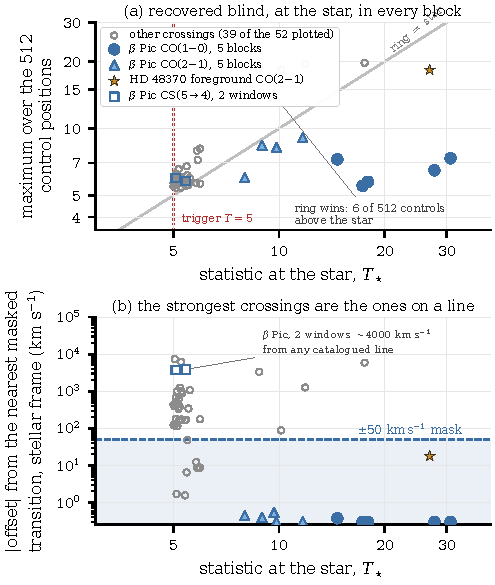
\includegraphics[width=0.88\columnwidth]{figures/bpic_control.pdf}
\caption{The $\beta$~Pictoris positive control, in both directions. Both
panels draw the same \BpicPanelNDrawn{} of the \NCross{} crossings, the
remainder having no retained control ring. \emph{(a)}~The spatial screen:
the stellar statistic against the maximum over that window's \NCtrl{}
control positions. Filled symbols are the blocks in which the blind search
recovers circumstellar carbon monoxide at $\beta$~Pictoris,
\NStageOneBpicEb{} of them with the star above every control and one with
the ring above it, block \texttt{\BpCtrlBlock}, Band~\BpCtrlBand, where the
ring reaches \BpCtrlRingMax{} against \BpCtrlStar{} at the star
(\S\ref{sec:bpicval}). \emph{(b)}~The same crossings by velocity offset
from the nearest masked transition \emph{in their own star's rest frame},
with the adopted $\pm\MaskHalfKms$\,km\,s$^{-1}$ half-width marked: the
\BpicPanelNCo{} $\beta$~Pictoris carbon-monoxide crossings land
\BpicDvCoLo--\BpicDvCoHi\,km\,s$^{-1}$ from CO, and its \BpicPanelNCs{}
CS($5{\to}4$) crossings \BpicDvCsLo--\BpicDvCsHi\,km\,s$^{-1}$ from anything
catalogued. \BpicPanelNOther{} further crossings are grey, HD~48370 marked.}
\label{fig:bpiccontrol}
\end{figure}
